%% ==============================
\chapter{Implementation}
\label{sec:implementation}
%% ==============================
Questions to ask:
\begin{enumerate}
    \item Which frameworks from others do you use? (open source tools)
    \item Which algorithms do you use?
    \item Which programming language do you use and why did you choose it?
    \item What code patterns did you apply?
    \item How does the most relevant part of your code work? (Pseudocode?)
    \item Which parameters can be used for configuration?
    \item How did you find the used set of parameters?   
    \item What are the interfaces for the end user?
    \item How to use your work?
\end{enumerate}

What is the software or hardware system used to implement the research ideas? 

Which frameworks or approaches from previous work are used? 

What are the main design choices and trade-offs in your system? 

What are the main implementation challenges and solutions? 

(If relevant) Which algorithms are used? (With pseudocode) 

The multi-floor navigation is implemented in Python 3.9 and later integrated into \gls{ros_2} Foxy. It is designed to be modular and can be easily integrated with the existing \gls{nav_2} stack. The planner is also designed to be scalable and can be used in environments of varying sizes and complexity. For the coordination of all subtasks the behavior tree library BehaviorTree.CPP \cite{auryn_robotics_behaviortreecpp_2023} is used. Single BT actions are programmed in C++ and it can easily be used to interact with ROS 2 nodes. The hierarchical planner is implemented in a different ROS 2 node entirely in Python. the most used libraries are NetworkX for building and planning in the graphs, OpenCV for gridmap handling and image segmentation and Shapely for the collision checks during roadmap generation and path planning. All of these libraries are efficiently implemented and use C-libraries under the hood to speed up the calculation. The code produced in this work is mainly done with Python as it is faster to prototype and well documented libraries for graph handling exist. This work does not claim to have a very efficient implementation or the best performance, it is meant only as proof-of-concept.

%% ==============================
\section{Hierarchy Creation}
\label{sec:hierarchy_creation}
%% ==============================
The input for hierarchy creation is the raw occupancy gridmap from the SLAMing process of the robot. For the evaluation and better comparison the same benchmark map as used for the algorithm from \cite{ryu_hierarchical_2020} is taken. For better readability the image of this raw occupancy gridmap from Chapter \ref{sec:benchmarks} is shown again here in Figure \ref{fig:freiburg_benchmark_2}.

\begin{figure}[h]
    \centering
    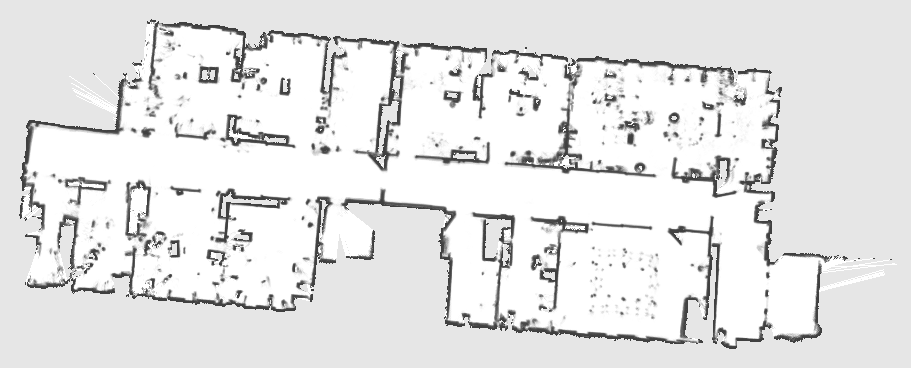
\includegraphics[width=0.75\textwidth]{figures/30_methods/freiburg_benchmark.png}
    \caption[The benchmark environment for hierarchy creation and straight path planning (intentional repetition)]{The benchmark environment for hierarchy creation and straight path planning recorded in the University of Freiburg (Source: \cite{cyrill_stachniss_robotics_2015})(intentional repetition)}
    \label{fig:freiburg_benchmark_2}
\end{figure}

This gridmap is build with the laser scanners of the mobile robot starting from the current pose at the time of starting the mapping. This starting pose is often not aligned with surrounding walls resulting in an apparent angle between the walls and the coordinate frame of the gridmap. This is not a problem for localization or path planning but makes it difficult to plan straight paths parallel to the walls. To solve this problem a rotation detection and outlier reduction algorithm is used.

\begin{figure}[h]
    \centering
    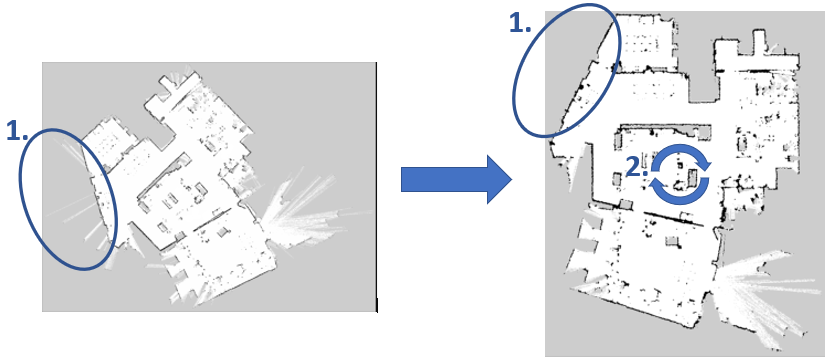
\includegraphics[width=0.75\textwidth]{figures/50_implementation/model_preprocessing_goal.png}
    \caption[Map preprocessing with rotation and outlier detection]{Map preprocessing with rotation and outlier detection. Original map on the left with outliers caused by transparent windows (1.). Resulting map on the right, outliers removed (1.) and rotation aligned with wall directions (2.) (Source: Tim Albert)}
    \label{fig:map_preprocessing}
\end{figure}

In Figure \ref{fig:map_preprocessing} the result of the preprocessing algorithm is seen. The algorithm first performs dilation and detects connected components. Based on the size these components are classified as outliers and the corresponding walls and white trails (see Figure \ref{fig:map_preprocessing} 1.) are removed. Then with the Probabilistic Hough Transform \cite{matas_robust_2000} straight lines are detected which represent the walls of the rooms. Finally the main orientation based on the most wall lines going in the same direction is chosen. To account for walls of one room and the adjacent wall perpendicular to it, the detected lines are clustered with the \gls{dbscan} algorithm \cite{ester_density-based_1996}. After obtaining the major rotation angle of the walls, the whole map is rotated to align with the coordinate frame of the gridmap. As this was developed and tested in an independent project it is not in the scope of this work.

The resulting map is now rotated parallel to the walls and outliers are removed. However there are still some artifacts in the map which obscure the real shape of the room. For best results some manual cleaning is still necessary. Most of these objects are dynamic obstacles which were at these positions during the mapping process but could be moved somewhere else by now. To not depend on this current snapshot of the environment the real shape of the room is estimated. The obstacles are later considered during the actual driving process. The task of the controller is to avoid these obstacles and provide a path around it. If this is not possible within the limits of the controller a replan is triggered. The resulting cleaned map is then binarized with a threshold and can bee seen in Figure \ref{fig:map_cleaned}

\begin{figure}[h]
    \centering
    
\includegraphics[width=0.75\textwidth]{figures/50_implementation/ryu.png}
    \caption[Binary map after rotation and manual cleaning]{Binary map after rotation and manual cleaning}
    \label{fig:map_cleaned}
\end{figure}

The segmentation of this map into single rooms and corridors is now done with the marker-controlled watershed algorithm \cite{parvati_image_2009}. For this the gridmap is converted into an numpy matrix and processed with opencv. OpenCV offers implementations for common image processing operations in python with which the watershed representation can be created. The process starts creating markers with which the normal watershed algorithm can be improved. Without predefined markers, watershed results in an over segmentation. For this an distance transform is performed on the image from Figure \ref{fig:map_cleaned}. This creates a mapping of each white pixels distance to the nearest black pixel. This can be interpreted as the obstacle clearance of this position and corresponds to the safety cost mask from Seder \cite{seder_hierarchical_2011}. By thresholding this distance map on a reasonable distance value d, the resulting binary image shows in white all pixels that have a distance greater or equal to d as seen in Figure \ref{fig:distance_transform}. Thus it represents the areas where most likely rooms are located. 

\begin{figure}[h]
    \captionsetup[subfigure]{justification=centering}
    \centering
    \begin{subfigure}{.5\textwidth}
      \centering
      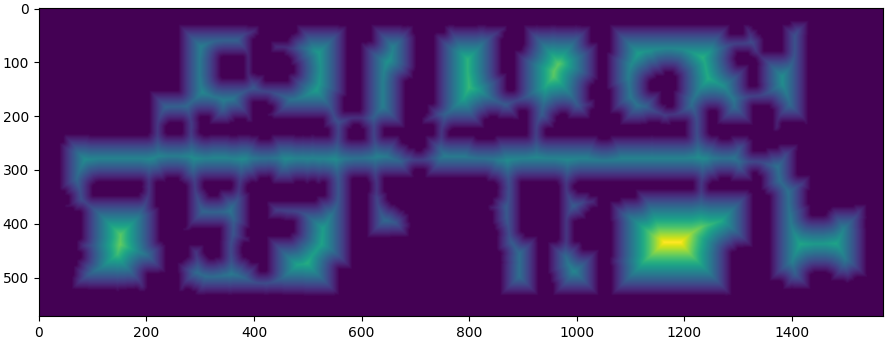
\includegraphics[width=\textwidth]{figures/50_implementation/ryu_distance_transform.png}
      \caption{Distance transform}
    \end{subfigure}%
    \begin{subfigure}{.5\textwidth}
      \centering
      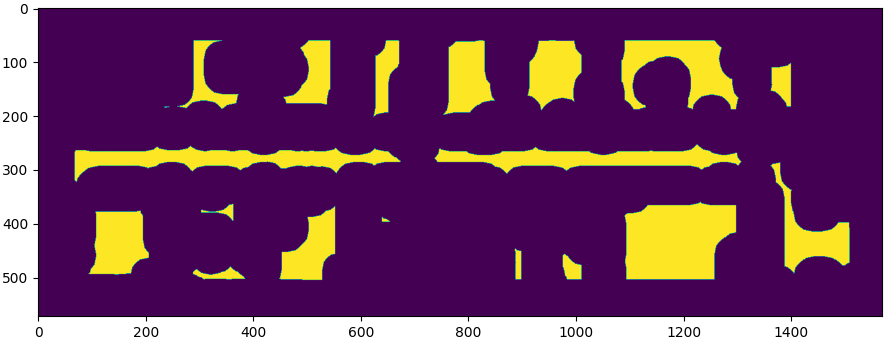
\includegraphics[width=\textwidth]{figures/50_implementation/ryu_markers.png}
      \caption{Markers as binary threshold of (a)}
    \end{subfigure}
    \caption[Distance transform and resulting markers]{Distance transform (a) and resulting markers (b) as initial information for the watershed algorithm.}
    \label{fig:distance_transform}
\end{figure}

To get the count, outlines and areas of each segment, the OpenCV function for detecting connected components is performed and returns a list of each area. With this list as input the watershed is then marker-controlled and provides a good segmentation of the whole floor into separate rooms as seen in Figure \ref{fig:watershed}.

\begin{figure}[h]
    \centering
    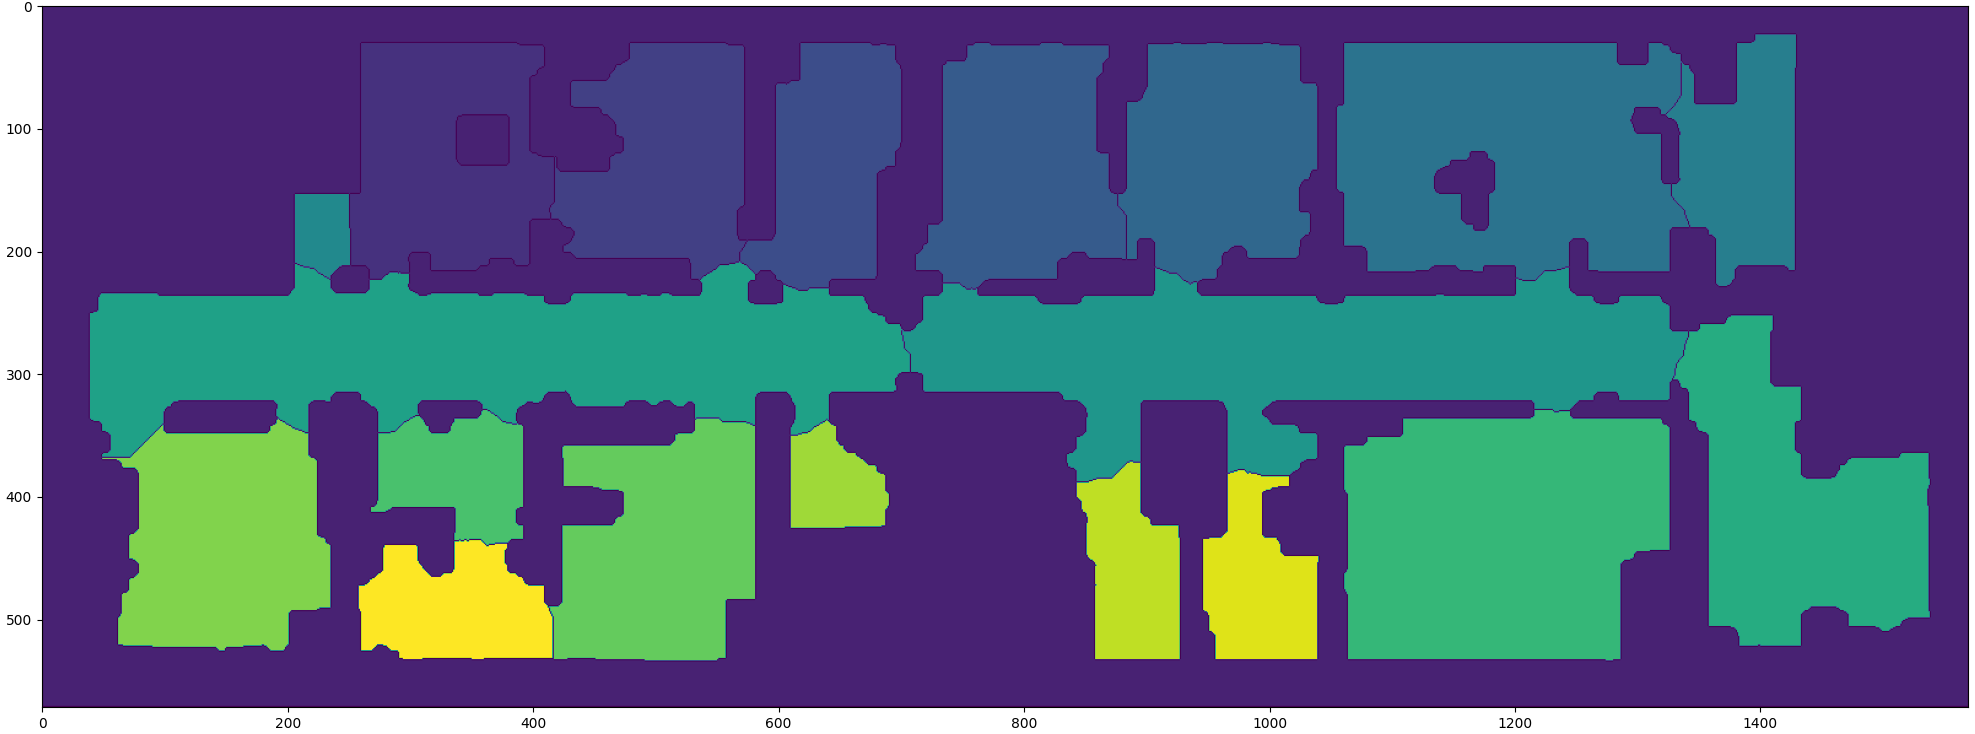
\includegraphics[width=0.75\textwidth]{figures/50_implementation/ryu_watershed.png}
    \caption[Marker-controlled watershed of the benchmark map]{Marker-controlled watershed of the benchmark map}
    \label{fig:watershed}
\end{figure}

This room segmentation provides the area for each room. To create a hierarchical graph from this the doors between them are important to create a hierarchical connection in the floor graph. The algorithm used in this work is based on the junction nodes extraction algorithm proposed by Ryu \cite{ryu_hierarchical_2020}. 

The base for this algorithm is the result of the watershed segmentation of Figure \ref{fig:watershed}. First, an adjacency matrix of the rooms are created. If rooms directly connect to each other with only a border created from the watershed in-between them, they have a real world connection. This connection and all pixels that lay on this border are stored. The distance transform from Figure \ref{fig:distance_transform} (a) is then taken to lookup the pixel with the maximum distance to the walls from that list of pixels on the border. Repeating this step for all connections in the adjacency matrix results in the bridge points with the maximum distance to the wall. 

\begin{figure}[h]
    \captionsetup[subfigure]{justification=centering}
    \centering
    \begin{subfigure}{.65\textwidth}
      \centering
      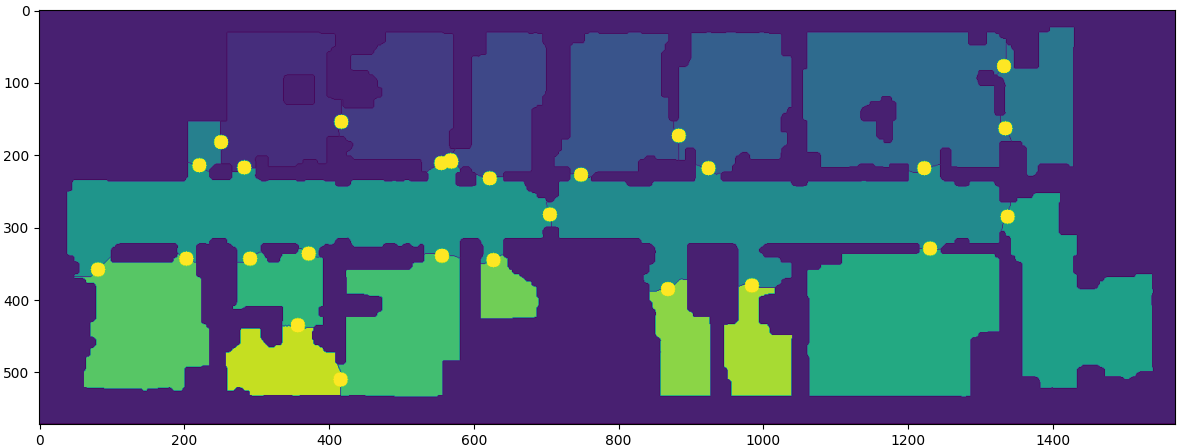
\includegraphics[width=\textwidth]{figures/50_implementation/ryu_bridge_nodes.png}
      \caption{Watershed result with detected bridge points}
    \end{subfigure}%
    \begin{subfigure}{.25\textwidth}
      \centering
      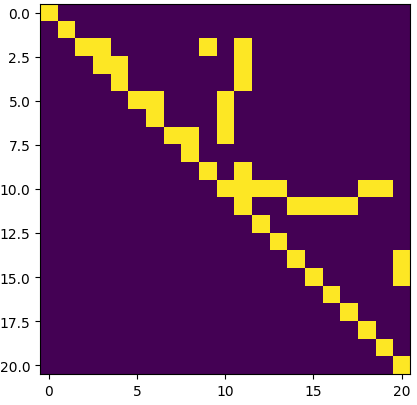
\includegraphics[width=\textwidth]{figures/50_implementation/ryu_adjacency_matrix.png}
      \caption{Adjacency matrix}
    \end{subfigure}
    \caption[The result of the bridge point detection algorithm]{The result of the bridge point detection algorithm. Bridge points overlayed on the segmented map (a). The adjacency matrix of the rooms (b). Rooms have always pixels connecting them to itself (diagonal line).}
    \label{fig:bridge_nodes}
\end{figure}

The segmented floor into rooms and their connections represented as bridge points can now be represented as a graph. Each room becomes a node in the floor graph. Each bridge point represents a door and becomes an edge in the graph. The corresponding graph can be seen in Figure \ref{fig:ryu_graph}. Note that this is inverted in the y-axis as all of the map previous images were taken from OpenCV which per default has its origin for images in the top left corner. In comparison, the graph representation is done with NetworkX which has its origin in the bottom left corner. 

\begin{figure}[h]
    \centering
    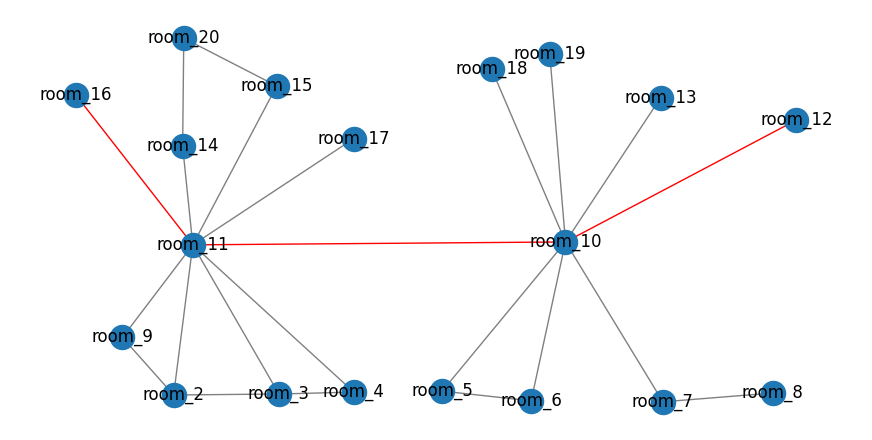
\includegraphics[width=0.7\textwidth]{figures/50_implementation/ryu_floor_graph.png}
    \caption[Graph representation of the benchmark map]{Graph representation of the benchmark map. Nodes are rooms and edges represent doors between them. In red is an example path from room 16 to room 12.}
    \label{fig:ryu_graph}
\end{figure}

To create an H-Graph for this benchmark, each room node has to hold a graph itself. These subgraphs are then the lowest hierarchical level and represent the roadmap of each room. Each Roadmap consits of collision free paths on the correspondign room-gridmap. To create this roadmap the straight path planner ILIR is used.


%% ==============================
\section{Roadmap Generation}
\label{sec:roadmap_generation}
%% ==============================
The first step for path planning is converting the environment in a Shapely object. This has the advantage, that basic shapes like lines, rectangles and polygons available, collision checks between these shapes are already implemented efficiently with a C library and the precision is higher than on the pixel based images. The images from OpenCV represent the environment in discrete pixels, this is helpful as the gridmap recorded from the laser scanners has exactly this resolution. However for collision checks and creating paths as lines it is important to precisely model these shapes. Lines should be one dimensional shapes which have no are. In comparison a line in an numpy matrix as used by OpenCV is represented in a row of pixels each with a certain width and height. This produces unexpected behavior and wrong results. The converted shapely environment can be seen in Figure \ref{fig:ryu_shapely}

\begin{figure}[h]
    \centering
    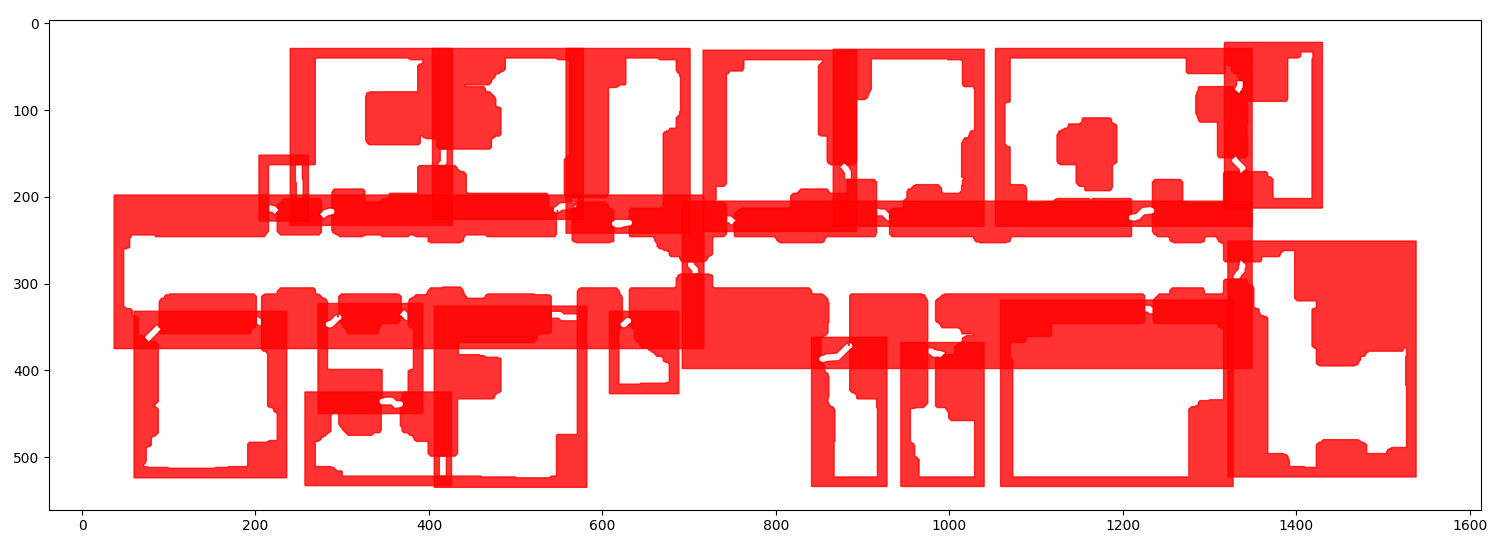
\includegraphics[width=0.75\textwidth]{figures/50_implementation/ruy_shapely.png}
    \caption[Shapely representation of the benchmark map]{Shapely representation of the benchmark map. Each room has its own environment and is surrounded by red obstacles. All room environments are drawn in one single image for visualization resulting in overlapped red obstacles.}
    \label{fig:ryu_shapely}
\end{figure}

In each room the largest interior rectangles are searched in an iterative process and combined to a polygon. The algorithm for finding the largest interior rectangle (LIR) is from Marzeh et. al \cite{marzeh_algorithm_2019} and the used python implementation from Weber \cite{weber_largest_2023}. The proposed Iterative Largest Interior Rectangle (ILIR) algorithm extends these ideas by repeatedly searching the largest rectangle. In Algorithm \ref{lst:pseudo_code_ilir} the pseudo code of the ILIR straight path planner is shown. In each room the LIR algorithm is executed (Line 14) and the found rectangle is later subtracted from the original area and the same process is repeated with the remaining area (Line 21). This produces not only the largest rectangle but also a polygon which is aligned to the axis of the coordinate frame. Just finding the largest interior polygon would not be useful as with high resolution this would just approximate the original shape. Also the edges of this polygon would not be parallel to the walls of the room which is an important requirement for the proposed algorithm. Additionally for each rectangle it is decided if the shape belongs either to a corridor or to a room based on predefined parameters (Line 16). For an corridor the rectangle is collapsed to a straight line to provide a better path for the robot. This process is repeated for each room until the area of the largest remaining contour is below a predefined threshold (Line 10). All paths are stored in list which is equivalent to the roadmap. Finally the found rectangles are merged to one polygon (Line 24) and the bridge points to other rooms are connected to it (Line 26).

\lstset{language=C++, mathescape=true, caption={Pseudo code of the ILIR straight path planner}, label={lst:pseudo_code_ilir}, morekeywords={from, to, is, Input, Output, each, in, end, do, then, Algorithm}}
\begin{lstlisting}[float=h]
Algorithm: Iterative Largest Interior Rectangle (ILIR)
Input: gridmap, parameter
Output: roadmap

room_list $\gets$ markerControlledWatershed(gridmap)

bridge_points $\gets$ extractBridgePoints(room_list)

for each room in room_list do:

    while largest_contour.area > parameter.min_area do:
    
        largest_contour $\gets$ maxContourByArea(room)
            
        largest_rectangle $\gets$ largestInteriorRectangle(largest_contour)

        if isCorridor(largest_rectangle) then:
            room.roadmap.add(centerLine(largest_rectangle))
        else
            room.roadmap.add(largest_rectangle)

        room $\gets$ (room - largest_rectangle)
    end

    room.roadmap $\gets$ mergeRectangles(room.roadmap)
    
    room.roadmap.add(connectBridgePoints(bridge_points))
end
\end{lstlisting}

In Figure \ref{fig:ilir_room_roadmap} the ILIR algorithm is applied on room 2 of the benchmark map. The red shapely environment represents the \(C\)-space for the path planning problem. The free area from (a) is converted into the \(C\)-space and a safety margin is applied with a dilation operation onto the walls and obstacles.  Therefor obstacles in the \(C\)-space look bigger than they are in the real world. This safety margin depends on the size of the robot and additional safety considerations. This allows to treat the robot as a dot in \(C\)-space and still ensure a collision free path. 

\begin{figure}[h]
    \captionsetup[subfigure]{justification=centering}
    \centering
    \begin{subfigure}{.235\textwidth}
      \centering
      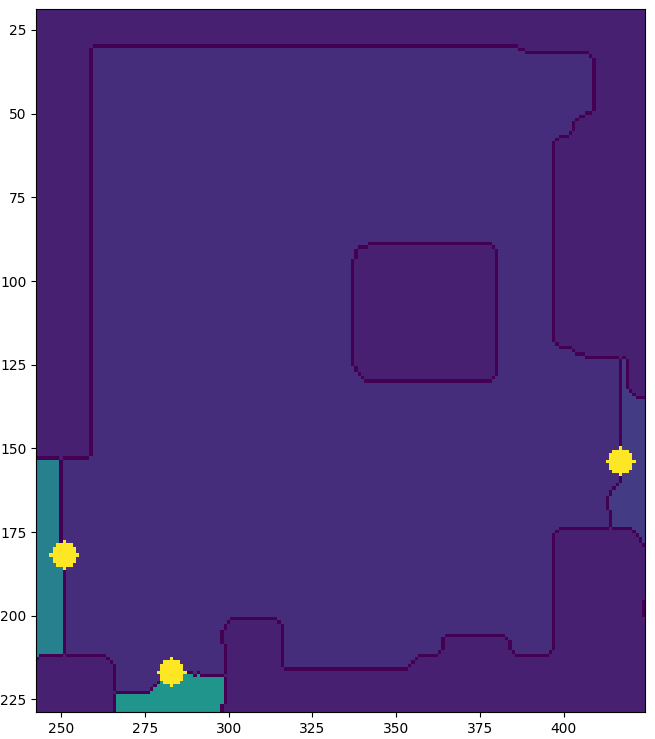
\includegraphics[width=\textwidth]{figures/50_implementation/ryu_room2_clean.png}
      \caption{Room after segmentation}
    \end{subfigure}%
    \begin{subfigure}{.25\textwidth}
      \centering
      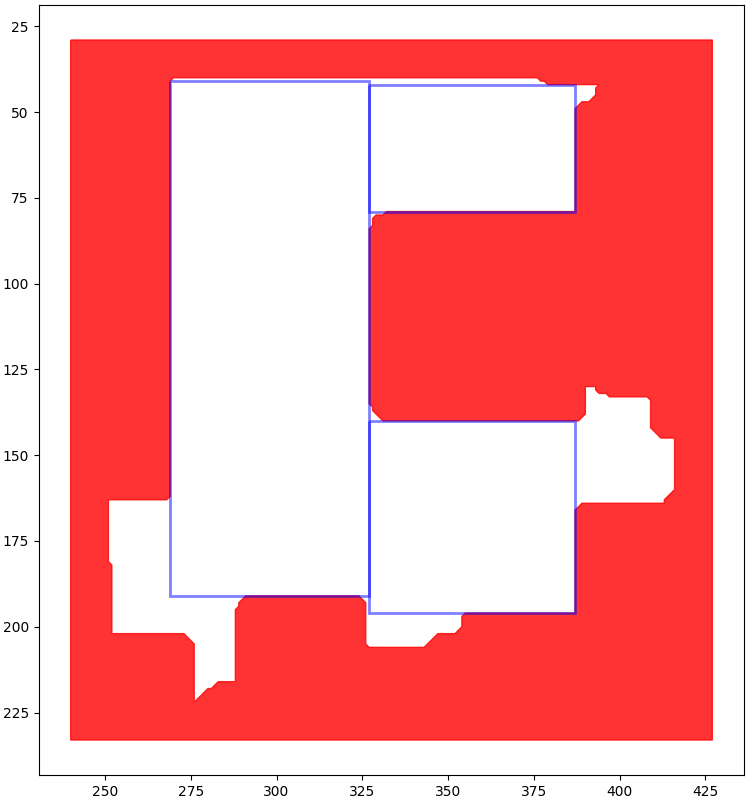
\includegraphics[width=\textwidth]{figures/50_implementation/ryu_room2_rectangles.png}
      \caption{Largest interior rectangles}
    \end{subfigure}%
    \begin{subfigure}{.25\textwidth}
      \centering
      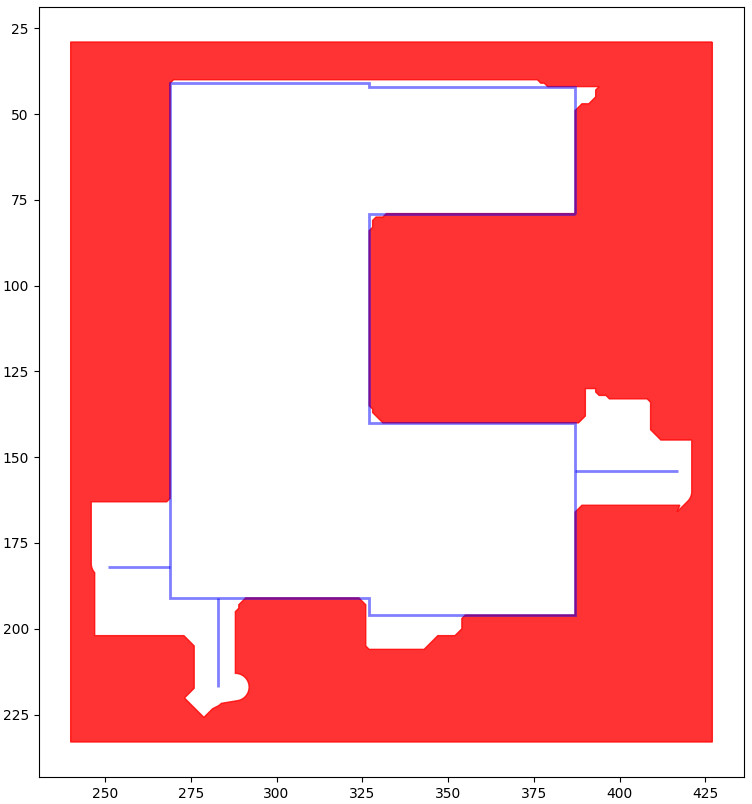
\includegraphics[width=\textwidth]{figures/50_implementation/ryu_room2_roadmap.png}
      \caption{Roadmap as produced by ILIR}
    \end{subfigure}%
    \begin{subfigure}{.25\textwidth}
      \centering
      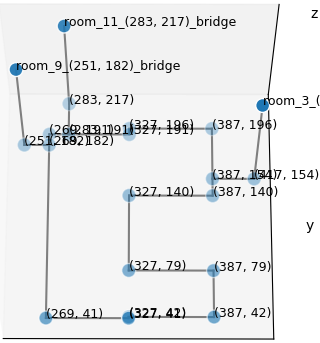
\includegraphics[width=\textwidth]{figures/50_implementation/ryu_room2_roadmap_graph.png}
      \caption{Roadmap converted to a graph}
    \end{subfigure}
    \caption[Application of the ILIR straight path planner on room 2 from the benchmark map]{Application of the ILIR straight path planner on room 2 from the benchmark map. The red obstacles are enlarged by the radius of the robot to ensure collision free paths. Note that the y-axis of the graph representation is inverted to the other images.}
    \label{fig:ilir_room_roadmap}
\end{figure}

As the last step of the ILIR algorithm, the door of neighbouring rooms are connected to the merged rectangles. In Figure \ref{fig:ilir_room_roadmap} (a) three doors to other rooms can bee seen as yellow points. These are then connected to the polygon and form the resulting roadmap in (c). These connections are created first by checking the direct straight line with the shortest distance between the door and the roadmap. If this line is in collision, an A* search is done to find the shortest possible connections. This resulting path from A* will then be smoothed and turned into a series of straight lines which are then added to the roadmap. For the actual path planning in the real world, the robot can be at an random valid position in the room and first has to find a collision free path to the roadmap before it can follow the roadmap the door of the next room or an elevator of the next floor. This connection of start and goal positions that or not on the roadmap is done by the same process and can bee seen in the next chapter in Algorithm \ref{lst:pseudo_code_ilir}. To make this roadmap searchable in a H-Graph it is converted to nodes and edges in the corresponding room graph (d). The connections in z-axis represent the hierarchical connections to another graph. They have no path cost and therefore will not be considered in the total distance of the path. By repeatedly applying the ILIR algorithm to each room in the previously segmented gridmap the levels H1 and H2 of the H-Graph can be automatically generated. In Figure \ref{fig:ryu_roadmap} a visualization of all the roadmaps of each room combined and overlayed on the image from the watershed is showed.

\begin{figure}[h]
    \centering
    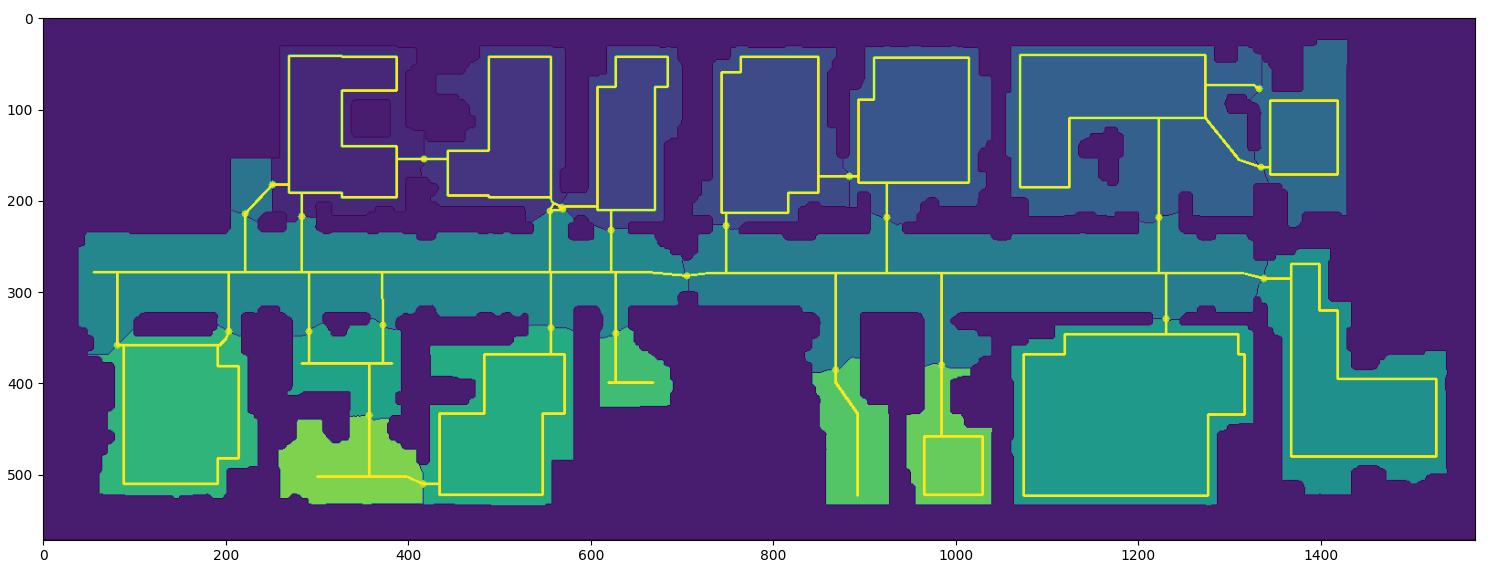
\includegraphics[width=0.75\textwidth]{figures/50_implementation/ryu_roadmap.png}
    \caption[Roadmap of the entire floor combined]{Roadmap of the entire floor combined and overlayed on the result from the watershed algorithm. It can be seen that paths in corridors are collapsed to a single line in the center.}
    \label{fig:ryu_roadmap}
\end{figure}

The ILIR algorithm is able to find a solution if a solution exists. This is ensured by the A* planner which is both complete and optimal. Thus the ILIR is also complete. However although the A* is used for bridge point connections the rest of the generated roadmap can not guarantee the shortest path. Thus the ILIR algorithm produces a path which is not optimal in terms of path length.

\todo{Zeitkomplexität}

%% ==============================
\section{Hierarchical Planning}
\label{sec:impl_hierarchical_planning}
%% ==============================
An overview of the different components for hierarchical path planning was given in Chapter \ref{sec:hierarchical_planning}. In Figure \ref{fig:h_graph_uml} a more detailed UML diagram of the H-Graph implementation is shown. The Coordinator and the Environment Model work as described in the concept. Here the focus is on the specific implementation of the H-Graph and its recursive hierarchical planning method.

\begin{figure}[h]
    \centering
    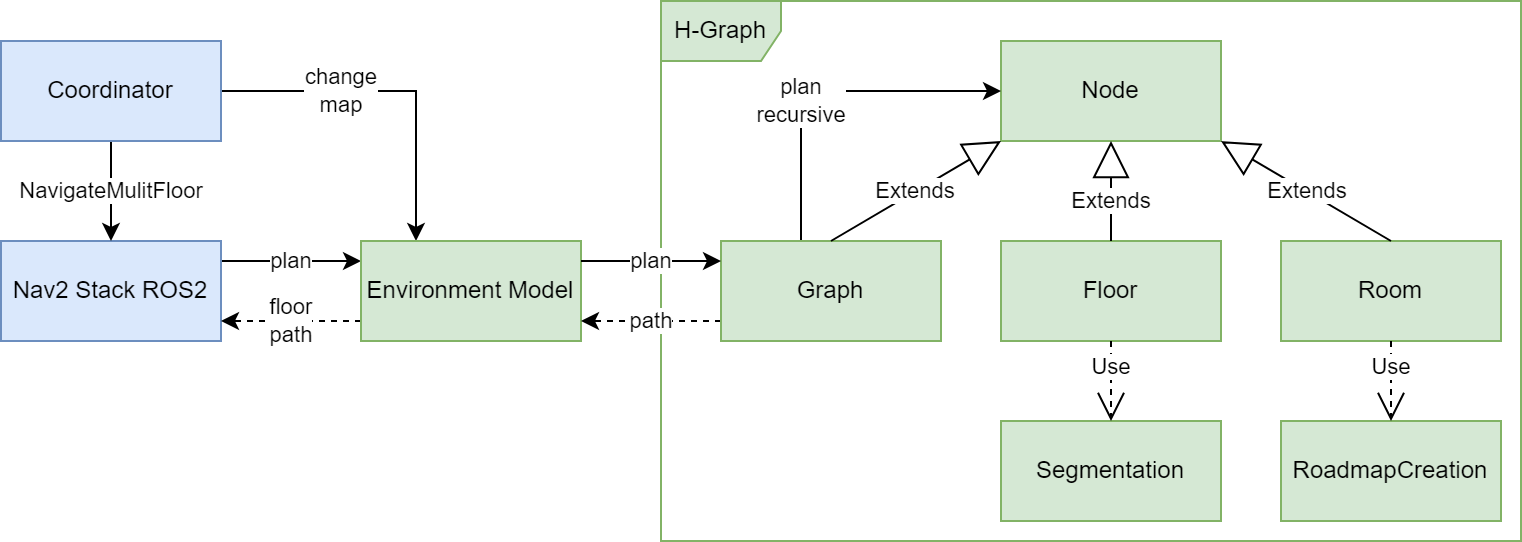
\includegraphics[width=\textwidth]{figures/50_implementation/h_graph_uml.png}
    \caption[UML diagram of the H-Graph implementation]{UML diagram of the H-Graph implementation. Blue components were taken from the community, green components were developed in this work.}
    \label{fig:h_graph_uml}
\end{figure}

The base class for each component in the H-Graph is the Node. This class implements all the basic functions needed to work as a hierarchically structured graph. This includes a private variable holding the corresponding subgraph of the next lower hierarchy. Each node of the subgraph is again from type of the base class Node. The public methods of Node are for adding and retrieving nodes and connections to the subgraph as well as one function to plan with Dijkstras algorithm in the subgraph and another function to plan recursively between arbitrary nodes in the H-Graph. This function is first planning the path in the subgraph and then handing over the planning process to each node in this path on the next lower hierarchy level. Details of the implementation of this recursive algorithm are shown in \ref{lst:pseudo_code_recursive}. To start this recursive planning process it has to be initialized with some values like the unique start and goal positions in the hierarchy and the initial path on the subgraph. This is done by the Graph class which inherits from Node and represents a specialisation of its functionality. This Graph node generally only occurs once as it resembles the root of the H-Graph, initializes recursive functions and provides some functions for visualization. The other specializations of Node are the Floor and Room classes. These of important to initially build he H-Graph from the gridmap data. The Floor class executes the segmentation process and creates the correct number of Room nodes in its subgraph. Every Room triggers the creation of the roadmap in its corresponding are from the segmented gridmap. As these specialisations all inherit from the base class Node they use the same recursive hierarchical planning process. In a H-Graph a finite amount of hierarchy levels can be created. The planning process still works the same and will find a solution if possible. Because a building or a whole campus have no special functions that are necessary to be separated from normal nodes they are not implemented as an own class. These nodes are just inserted as plain Node objects into the H-Graph, the same as for bridge nodes which are only necessary for the planning process.

\lstset{language=C++, mathescape=true, caption={Pseudo code of Hierarchical Path Planning}, label={lst:pseudo_code_planning}, morekeywords={from, to, is, Input, Output, each, in, end, then, Algorithm}}
\begin{lstlisting}[float=h]
Algorithm: Hierarchical Path Planning
Input: start_hierarchy, goal_hierarchy, h_graph
Output: path

for hierarchy in [start_hierarchy, goal_hierarchy] do:

    room, pos $\gets$ getHierarchyH2(hierarchy)
    
    if pos not in room.roadmap then:
    
        if noCollision(straightLine(pos, room.roadmap)) then:
        
            path $\gets$ straightLine(pos, room.roadmap)
            
            room.roadmap.add(path)
        else:
            path $\gets$ A*Planner.plan(pos, room.roadmap)
            
            room.roadmap.add(path)
end

path $\gets$ RecursiveHierarchicalPlanner.plan(
            start_hierarchy, goal_hierarchy, h_graph)

\end{lstlisting}

The first step of the whole navigation process is the trigger from the Coordinator to the \gls{nav_2} stack which hands it to the responsible planner plugin. This is the custom Hierarchical Planner which then sends a ROS 2 action goal to the environment node. The interfaces of the process up to there is later presented in the next chapter \ref{sec:multi_floor_behavior_trees}. At this point the ROS 2 action server of the Environment Model node starts the hierarchical planning. This process is shown in the Algorithm \ref{lst:pseudo_code_planning}. The path planning starts by first checking if the given start and goal positions are already in the roadmap of the corresponding room (Line 9). If they are not in the roadmap, they first have to be connected with a path. For this, the straight line between the position the the closest point in the roadmap is checked for collision (Line 11). If this line is free, the connections is added to the roadmap and therefor the position is now part of the subgraph and can be searched by the following planning process. If the straight line connection should not be possible because of an obstacle, the shortest path around it is searched with the A* algorithm (Line 17). This is guaranteed to find a solution path if it is possible. After both, the start and the goal location, have been added to the roadmap it is now possible to find the solution by searching the H-Graph. As these locations could be on very different parts of the environment and therefor on different branches of the hierarchical structure, the proposed recursive hierarchical planner is needed to search through every hierarchy of the H-Graph. This process is later described in Algorithm \ref{lst:pseudo_code_recursive}.

\lstset{language=python, mathescape=true, caption={Unique H-Graph positions and path representation}, label={lst:pseudo_code_datastructure}, morekeywords={from, to, is, input, output, each, in, end}}
\begin{lstlisting}[float=h]
# general description of a unique position:
$p = \{p_{Hn}, p_{Hn-1}, ..., p_{H1}\}$

# specific unique position with 4 hierarchies in Python:
p_hierarchy = ["Building F", "Floor 2", "Room 2", (50,210)]

# specific example path with 4 hierarchies in Python:
path = {
    "Building F": {
        "Floor 3": {
            "Meeting Room": {...},
            "Corridor": {...},
            "Elevator": {...},
            "Floor 2_Elevator_bridge": {}
        },
        "Floor 2": {
            "Floor 3_Elevator_bridge": {},
            "Elevator": {...},
            "Corridor": {...},
            "Terrace2": {...},
            "Terrace_Floor 1_Ring F_bridge": {}
        },
        "Terrace_Floor 1_bridge": {}
    },
    "Terrace": {
        "Building F_Floor 2_bridge": {},
        "Floor 1": {
            "Building F_Floor 2_Terrace2_bridge": {},
            "Ring F": {...}
        }
    }
}
\end{lstlisting}

But first the datastructure of such an unique hierarchical position and the path through the H-Graph has to be explained. In Algorithm \ref{lst:pseudo_code_datastructure} the general description of a unique position in the H-Graph can bee seen (Line 2). The position consists of the specific nodes of each subgraph for all hierarchies from top (\(Hn\)) to bottom (\(H1\)). As an example the unique description of a position in a 4 level H-Graph is shown in Line 5. The highest hierarchy level are buildings and the lowest is the specific position on the gridmap. As the node in for NetworkX can have any hashable value, a tuple for the position is used. The datastructure of a whole path through the H-Graph is shown in Line 8-32. For the reason of better visibility the lowest hierarchy (\(H1\)), the positions on the gridmap, is left out as the general structure is also made clear with the top three levels. The path is represented as a nested dictionary, Each entry in the dictionary has a key, the node in the path of the current hierarchy level, and a value which is another dictionary containing the path on the subgraph of the key node. Note that bridge nodes do not have an subgraph of their own as their or only for connecting the hierarchies. As of Python 3.7 dictionaries are guaranteed to keep the insertion order. This enables it to store the nodes in the right order as the are on the actual path. 

\lstset{language=C++, mathescape=true, caption={Pseudo code of the recursive planning function}, label={lst:pseudo_code_recursive}, morekeywords={from, to, is, Input, Output, each, in, end, then, enumerator, Algorithm, with}}
\begin{lstlisting}[float=h]
Algorithm: recursiveHierarchicalPlanning
Input: child_path, start_hierarchy, goal_hierarchy, hierarchy_level
Output: path

for node in child_path with enumerator i do:

    if isLeaf(node) or isBridge(node) then:
        path[node] $\gets$ {}
        continue

    if node is child_path[-1] then:
        child_graph_goal $\gets$ goal_hierarchy[hierarchy_level+1]
    else:
        child_graph_goal $\gets$ getBridgeTo(node, child_path[i+1])
        
    if node is child_path[0] then:
        child_graph_start $\gets$ start_hierarchy[hierarchy_level+1]
    else:
        child_graph_start $\gets$ getBridgeTo(node, child_path[i-1])

    next_child_path $\gets$ node.planInChildGraphWithDijstra(child_graph_start, child_graph_goal)

    path[node] $\gets$ node.recursiveHierarchicalPlanning(next_child_path, start_hierarchy, goal_hierarchy, (hierarchy_level+1))
end

return path
\end{lstlisting}

The hierarchical planning itself takes place inside the graph structure of the H-Graph as described in Figure \ref{fig:h_graph_uml}. The specialized Graph nodes initializes the search and then a recursive search over all relevant nodes takes place. This search process is shown in Algorithm \ref{lst:pseudo_code_recursive}. The inputs for this method are the unique start and goal positions, called \texttt{start\_hierarchy} and \texttt{goal\_hierarchy}, as well as the initial path \texttt{child\_path} in the root level subgraph created by the Graph node with a Dijkstra search. The given \texttt{hierarchy\_level} will always be counted up as the recursion progresses deeper. The algorithm now iterates through every node in the given path and triggers its own recursive planning function one hierarchy level deeper. If the last level is reached, the nodes do not have a subgraph anymore and therefor have the condition of a leaf node. This is checked in Line 7. The recursion also stops once a bridge node is reached as it also has no subgraph. During planning the corresponding path structure as a seen in Algorithm \ref{lst:pseudo_code_datastructure} is built. The dictionary is the filled with the current node as the key and an empty dictionary as the value indicating the end of recursion in this branch (Line 8). Instead if the node has a subgraph planning has to continue in this graph. For this the next start and goal positions of the child graph have to be found. If the current node is the goal node of the current path (\texttt{child\_path[-1]}), this means that the unique goal position is on this branch of the H-Graph and the goal node in the next subgraph one hierarchy level deeper is also defined in the unique goal position and can easily be extracted from it by \texttt{goal\_hierarchy[hierarchy\_level+1]} (Line 12). If this is not the case, this means planning has already progressed into the path on the current graph and all start and goal nodes one level deeper have to be bridge nodes connecting for example rooms or floors together. The name of this bridge node is determined by the current node and the next node in the path of the current graph (Line 14). The same has to be done for the start position on the subgraph and with that information the next path on the subgraph of the current node can be planned (Line 21). This is done again with a normal path planning algorithm like Dijkstra. Now, to close the loop for recursion, with this new subgraph, the same function is called again (Line 23). The result from this call is then also stored in the path dictionary with the current node as key and the whole subtree produced by the recursion as value. Finally once all nodes in the path of the current hierarchy level are finished planning, the produced dictionary is then returned one level higher and in the end back to the Graph node which started the process. 

The proposed algorithm for hierarchical planning in the H-Graph is both complete and optimal. This means if a solution exists it will be found and the found solution will be the best one in terms of path length. The reason for that is the Dijsktra algorithm used on each level for planning in the current graph. The hierarchical recursive search around it only ensures that the correct start and goal positions based on the current hierarchy level are chosen. Note that this algorithm can be used for an arbitrary problem with a H-Graph as base. It is not bound and limited to path planning. Although the application here is only for path planning. And in this specific case the available nodes in the subgraph of each rooms are limited by the nodes created on the roadmap. As the roadmap does not produce optimal paths on the given gridmap it can not yield the optimal path in the real worlds. As a consequence the combination of the straight path planner ILIR and this hierarchical planning is not optimal but still complete. As this is an intentional condition of the roadmap it works as expected and fulfills the goals for path planning of this work.

\todo{Time complexity of Dijstra and recursion}

% https://stackoverflow.com/questions/13467674/determining-complexity-for-recursive-functions-big-o-notation

% Bounds of the running time of Dijkstra's algorithm on a graph with edges {{mvar|E}} and vertices {{mvar|V}} can be expressed as a function of the number of edges, denoted <math>|E|</math>, and the number of vertices, denoted <math>|V|</math>, using [[big-O notation]]. 
% The simplest version of Dijkstra's algorithm stores the vertex set {{mvar|Q}} as a linked list or array, and edges as an [[adjacency list]] or [[Adjacency matrix|matrix]]. In this case, extract-minimum is simply a linear search through all vertices in {{mvar|Q}}, so the running time is <math>\Theta(|E| + |V|^2) = \Theta(|V|^2)</math>.

% For [[sparse graph]]s, that is, graphs with far fewer than <math>|V|^2</math> edges, Dijkstra's algorithm can be implemented more efficiently by storing the graph in the form of adjacency lists and using a [[self-balancing binary search tree]], [[binary heap]], [[pairing heap]], or [[Fibonacci heap]] as a [[priority queue]] to implement extracting minimum efficiently. To perform decrease-key steps in a binary heap efficiently, it is necessary to use an auxiliary data structure that maps each vertex to its position in the heap, and to keep this structure up to date as the priority queue {{mvar|Q}} changes. With a self-balancing binary search tree or binary heap, the algorithm requires
% :<math>\Theta((|E| + |V|) \log |V|)</math>
% time in the worst case (where <math>\log</math> denotes the binary logarithm <math>\log_2</math>); for connected graphs this time bound can be simplified to <math>\Theta( | E | \log | V | )</math>.  The [[Fibonacci heap]] improves this to
% :<math>\Theta(|E| + |V| \log|V|).</math>

%% ==============================
\section{Multi-Floor Navigation with Behavior Trees}
\label{sec:multi_floor_behavior_trees}
%% ==============================
The final steps for executing the multi floor navigation is coordinating the process with a behavior tree. This is done in the Coordinator ROS 2 node as seen in Figure \ref{fig:h_graph_uml}. The default action interface (introduced in Algorithm \ref{lst:navigatetopose.action}) expects a goal pose defined int he current map frame. Every default planner plugin would reject a goal which is not on the default "map" frame. As for multi-floor navigation it is necessary to specify a goal pose which is on another floor or building. To account for that the custom planner plugin proposed in this work handles the given frame different. It allows for custom frames which represent a unique floor position in the H-Graph. It is checked if this floor exists and then the an new action sends a goal to the Environment Model node which then triggers the planning function from Algorithm \ref{lst:pseudo_code_planning}. To ensure seamless integration into the current \gls{nav_2} stack, the frame id of all the poses in the returned path is changed back again to "map". If a floor changes happened, the BT has changed the current map on the map server and the positions are always valid on the new map.

\begin{figure}[h]
    \centering
    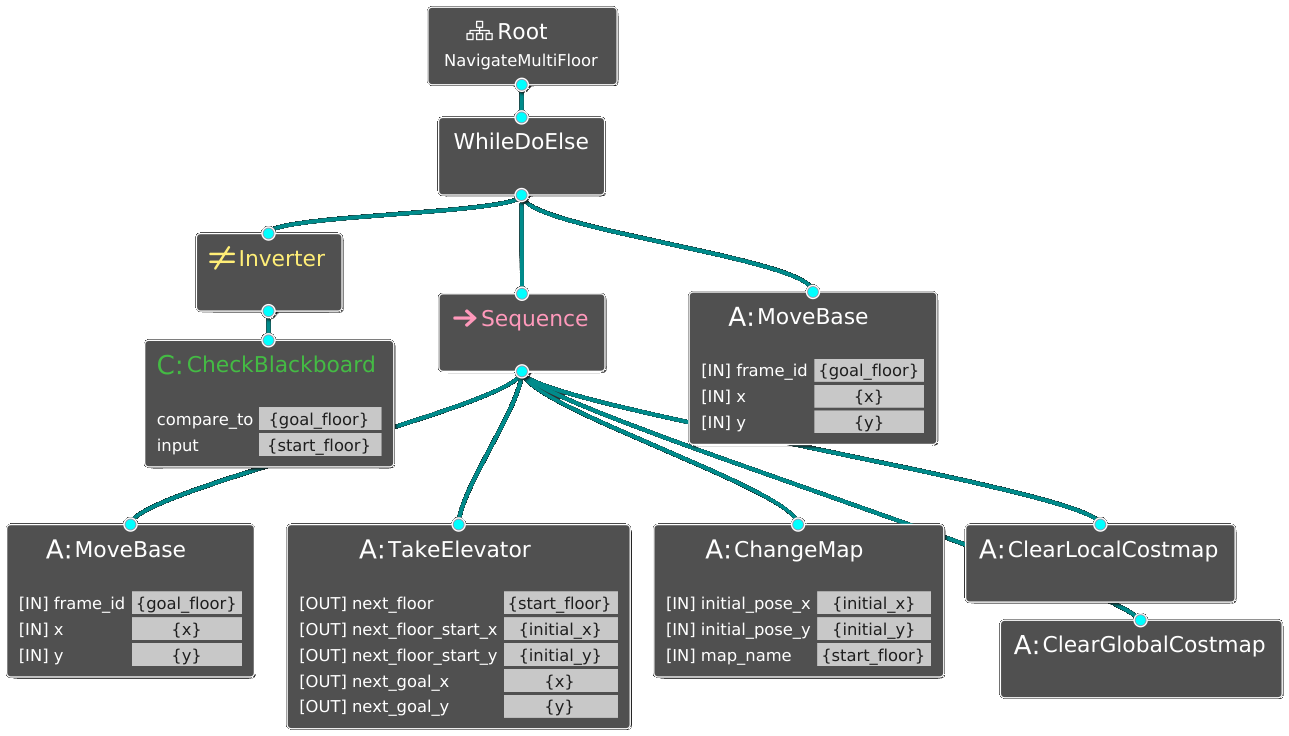
\includegraphics[width=\textwidth]{figures/50_implementation/bt_navigate_multi_floor.png}
    \caption[BT of the multi-floor navigation]{BT of the multi-floor navigation}
    \label{fig:bt_navigate_multi_floor}
\end{figure}

In Figure \ref{fig:bt_navigate_multi_floor} the behavior of one single multi-floor navigation process is shown. First in the WhileDoElse control node the left branch is checked as the break condition. As long as the break condition is true the middle branch is executed, if it is false the right branch is executed and the while loop is ended and therefor the whole subtree. The condition checks if the current floor value stored in the \texttt{start\_floor} variable is the same as the \texttt{goal\_floor}. The result of this check will then be inverted and used as the break condition of the while loop. This means as long as the floor are different the middle branch is executed and if the robot reaches the same floor as the goal floor the right branch is executed one single time. The sequence in the middle triggers all its children from left to right and executes a full floor change. Starting with the MoveBase action which call the action interface of the \gls{nav_2} stack. This uses the \texttt{goal\_floor} as frame\_id as described in the section above. The x and y coordinated of the goal for this action are also describing the goal position on the goal floor. Note that the custom planner plugin will always return only the part of the path that is on the current floor. As the hierarchical path of the H-Graph knows which elevator to take to reach the goal floor in the shortest distance it will determine the position that is given back to the \gls{nav_2} stack and executed by the robot. After the movement action the robot stand in front of the elevator. The next step is to trigger the necessary actions to perform this elevator transport. As discussed earlier in simulation this is only a teleport and for the PeTRA use-case this will be a complete subtree coordinating the movement of the arm to press the right buttons inside the elevator. The output of that action is next floor to which the robot has to drive, the initial position on the map of this new floor as well as the goal position on that floor. Depending on the hierarchical path this can be the final goal or another elevator position which causes the WhileDoElse to loop again. Next, the map has to be changed and the initial pose of the robot set. Before planning on this new map the cached local and global costmaps of the old floor have to be cleared. Once this is done the Condition is evaluated again and it either performs another map change or the final floor is reached and the MoveBase to the last goal pose is executed. With this goal pose reached the loop is ended and the behavior tree finished successfully.